\chapter{Event Reconstruction And Simulation}\label{ch:chapter3}
The detector provides information about the collisions and the underlying physics processes in the form of various electronic signals.
A number of steps have to be followed in order to obtain a meaningful physics result,
by making use of scientific and theoretical knowledge, computing and man-power. A diagrammatic representation of an event processing chain
in presented in \fig{\ref{fig:EvtChain}}.

\begin{figure}[h]
\begin{center}
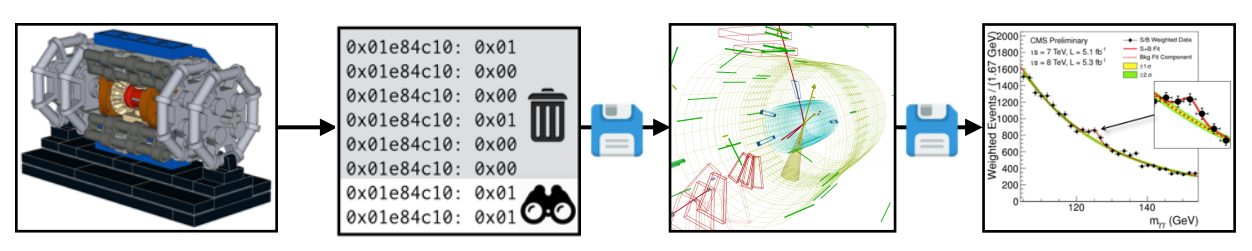
\includegraphics[width=15cm]{Chapter3/Event_reco_chain.png}
\caption{A diagrammatic representation of an event processing chain.}
\label{fig:EvtChain}
\end{center}
\end{figure}
\vspace{-0.2in}

The electronic signals from various sub-detectors are stored, after digitization, in the form of RAW data using online trigger and DAQ system.
This RAW data is further processed using a software based multi-level process, known as ``Event Reconstruction''~\cite{Lange:2011zza}, that refines the data,
applies various calibration corrections and construct high-level physics objects\footnote{High-level physics objects are the reconstructed particles like photons,
  electrons, muons, taus etc.}. At CMS, two levels of reconstruction are performed, one is a fast reconstruction, known as prompt reconstruction, done alongwith
the data collection by using less time consuming algorithms and the second one is a detailed reconstruction, known as re-reconstruction, performed at a later time.
The reconstructed data is written in various data formats (e.g. RECO, AOD, mini-AOD)
that differ in size, technicalities, compactness etc.

Based on the theoretical knowledge, it is possible to simulate the behaviour of various particles within the detectors using event generators, also
called Monte Carlo (MC) generators~\cite{Buckley:2011ms, Dobbs:2004qw}. Event generators make use of some computer programs based on Monte Carlo
techniques~\cite{MC_Tech} to generate physics events corresponding to different physics processes. This simulated data form an integral part of
any physics analysis, used in determining various SM parameters, validating$/$rejecting any new theory, forming expected background for experimental data,
evaluating various uncertainties and trigger parameters etc. In the language of statistics, it forms the null hypothesis for the test of any new theory. 
The simulated data is also written in different data formats like RECOSIM, AODSIM, mini-AODSIM, in correspondence with reconstructed data.

This chapter details the different steps and procedures used in the reconstruction and simulation of the events for CMS physics analyses.
\section{Event Reconstruction}
Reconstruction is the process of constructing physics quantities using the raw data collected from the experiment. 
Inside the CMS detector, starting from the collision point, the particles first arrive in the tracker where the charged particle's trajectories, their momenta and
interaction points are reconstructed using the particle's signal and bending angle in the sensitive layers of tracker. If the particle is either electron or photon,
it will be absorbed in ECAL. The EM showers generated by such particles are detected as energy clusters in ECAL cells and are used in the determination
of energy and direction of these particles. Hadrons (charged and neutral) will be absorbed in HCAL, sometimes initiating their showers in ECAL.
The associated clusters are used in measuring the energies and directions of hadrons. Only muons and neutrinos pass through the calorimeters with negligible interactions.
While neutrinos escape unidentified, muons leave their signature in muon detectors, used to reconstruct the muon direction and momentum.
This behaviour of different particles is graphically depicted in \fig{\ref{fig:CMS_slice}} in a slice of CMS detector.

\begin{figure}[h]
\begin{center}
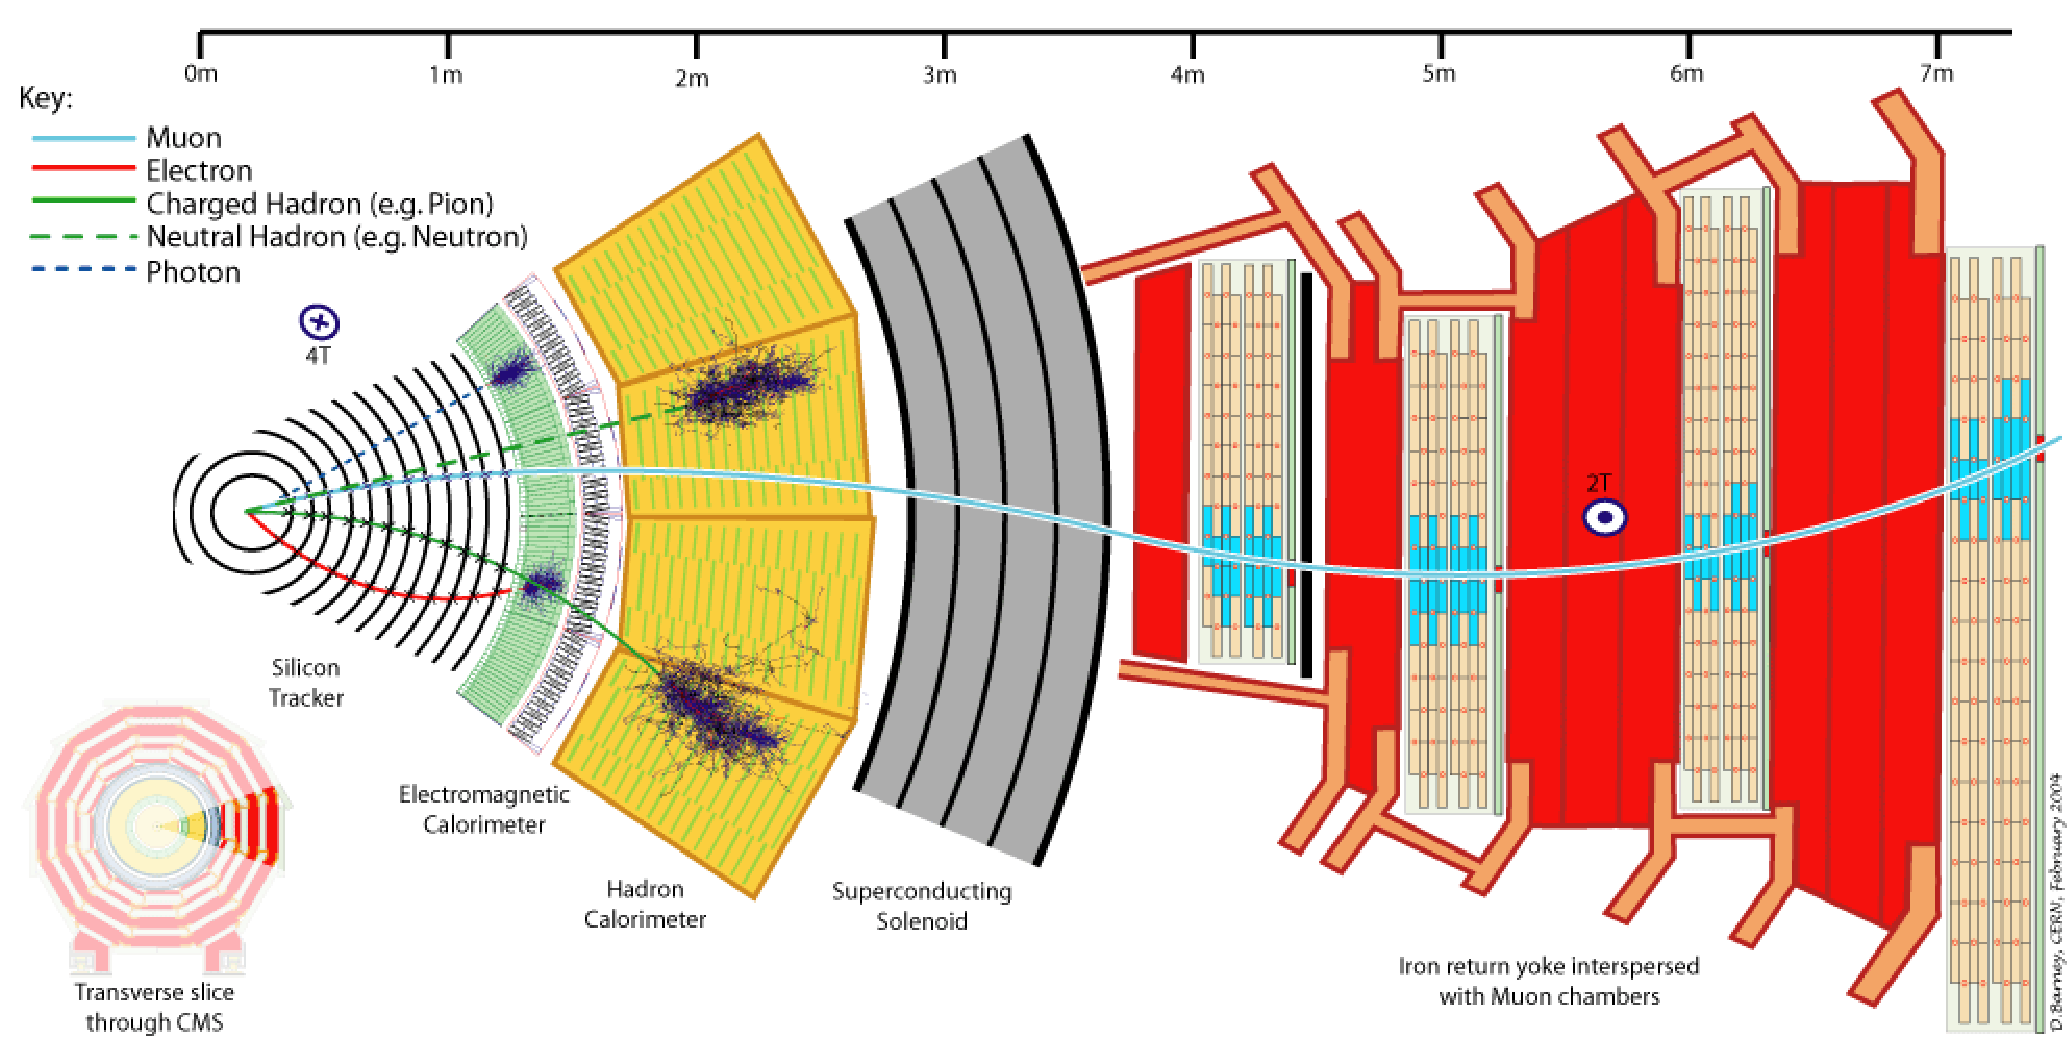
\includegraphics[width=14cm]{Chapter3/CMS_Slice.pdf}
\caption{A graphical representation of the trajectories of various particles through the CMS detector.}
\label{fig:CMS_slice}
\end{center}
\end{figure}

The CMS reconstruction software~\cite{Lange:2011zza} is a collection of several independent units, each consisting of many reconstruction algorithms
and provides one set of reconstructed objects at the output. The software has been developed and validated by making use of simulated data.
The complete reconstruction process is divided into three steps as shown in \fig{\ref{fig:CMS_reco_steps}}. 

\begin{figure}[h]
\begin{center}
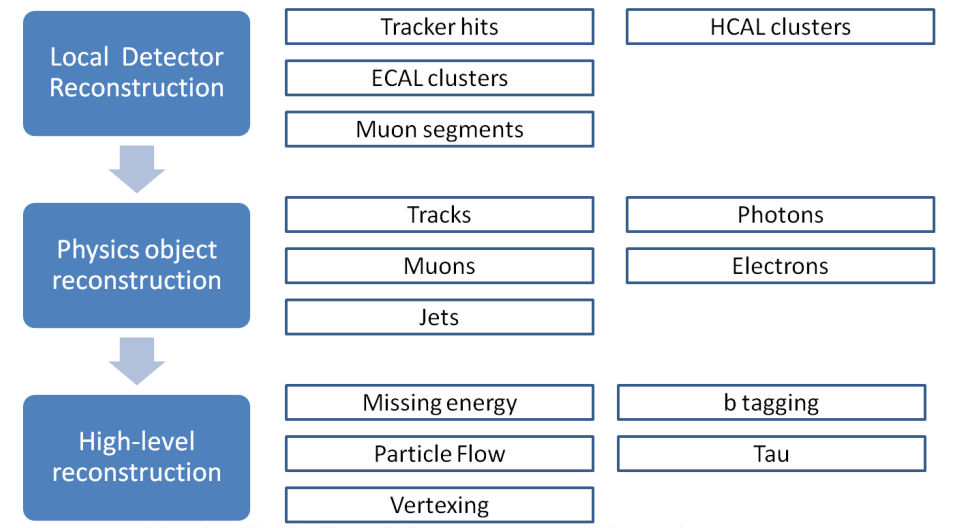
\includegraphics[width=12cm]{Chapter3/CMS_Reco_steps.png}
\caption{Different steps of CMS reconstruction program.}
\label{fig:CMS_reco_steps}
\end{center}
\end{figure}
\vspace{-0.2in}
At first, the local reconstruction takes place within a particular detector module of a sub-detector.
It uses raw data as input and provide in output the reconstructed units,
also called rechits. These rechits are corrected for any uncertainties by the application of different calibration corrections. 
The form of these rechits depends on the sub-detector under consideration. These are the position measurements inside tracker and muon system while
energy clusters inside the calorimeters. These reconstructed hits act as input to the next reconstruction level, known as global reconstruction
where the physics object reconstruction takes place. At this level, the information obtained from different detector modules within a sub-detector
is combined to form sub-detector level objects, like high$/$low $\pt$ charged particle tracks and displaced vertices in the tracker,
candidate muon tracks in the muon system, photon/electrons in ECAL and jets in ECAL$+$HCAL.
These objects from different sub-detectors are then combined to reconstruct high-level physics analyses objects
using an optimally efficient Particle Flow (PF) reconstruction algorithm~\cite{Sirunyan:2017ulk},
as a final stage of event reconstruction. 
The high-level objects like $\met$, tau, b-tagging $\etc$ that require the additional knowledge of
tracks, displaced vertices, $\sum{\pt}$, are also reconstructed at this level. 

Since this thesis is based on an analysis that requires a photon and a jet or a b-jet in the final state, so only the steps needed to reconstruct photons and
jets (b-jets) are considered in detail in the following sections.

\subsection{Track reconstruction}
The tracker is the first detector in which the charge particles leave their signatures, hence reconstruction of tracks is one of the most important task of
the CMS reconstruction program. More than a thousand particles pass through the tracker every 25\unit{ns}, thereby, making the track reconstruction
immensely challenging. The track reconstruction is a combinatorial kind of problem, as for a partial track formed by hits in the internal layers, there can be many
compatible hits forming different tracks in the outer layers, so the reconstruction algorithm should be able to properly locate the equitable hits without
loosing any tracks, over a broad range of $\pt$ from 100\unit{MeV} to 1\unit{TeV}. This insurmountable feat is achieved by the use of the
``Combinatorial Track Finder'' (CTF)~\cite{Chatrchyan:2014fea,Adam:934067} algorithm which is an extension of the
Kalman filter~\cite{Fruhwirth:1987fm, Billoir:1989mh, Billoir:1990we} algorithm, an algorithm that allows single framework
modelling of complete track reconstruction program. 
 
At first, the individual hits in pixel and strip tracker are reconstructed at the local reconstruction level by clustering the
zero-suppressed\footnote{Zero-suppression is the default noise cleaning performed in CMS detector, in which all signals below a particular threshold
are rejected, the value of the threshold depends on the sub-detector part under study.} signals passing
the specified thresholds. The corresponding hit positions and associated uncertainties are also estimated with an average efficiency of more than 99$\%$.  
These hits are then used as input into the CTF algorithm to reconstruct the charged particle tracks and their position$/$momentum. The CTF algorithm is based on
a process known as ``iterative tracking'' that reconstruct the track collection in a number of iterations. The basic idea is to first sort out the easily accessible
tracks, like the high $\pt$ ones near the interaction region and do not consider the hits corresponding to these tracks in the next iterations, thereby,
successively reducing the complexity of subsequent iterations. This strategy is very useful in building up of more difficult tracks,
like low $\pt$ or displaced tracks. The algorithm has a total of $6$ iterations, starting with iteration $0$, that reconstruct the prompt tracks
(close to pp interaction point) with $\pt$ $>$ 0.8\unit{GeV} and having at least three pixel hits.
Iteration $1$ takes care of all other high $\pt$ prompt tracks with two pixel hits. Iteration $2$ has been configured to locate low $\pt$ ($\pt$ $\le$ 0.8\unit{GeV}) prompt
tracks. Lastly, the iterations $3-5$ are intended to recover tracks originated outside the luminous region of pp interactions and not considered in previous iterations.
The first three iterations of CTF has a prompt track reconstruction efficiency of $\sim$ 90$\%$ for charged hadrons and $\sim$ 99.5$\%$ for muons, the
efficiency for hadrons deteriorate due to their nuclear interactions with the tracker material. The track reconstruction is the most CPU extensive
task with each iteration step constituted of four further steps as detailed below:
%\vspace{-0.1in}
\begin{itemize}[leftmargin=*]
\item {\bf{Seed generation}}: In this step, the track seeds are generated using the hits in the internal pixel layers of tracker. A set of parameters are used to determine
  the compatible hits that has the capability of track formation. Usually, a window around a hit in a layer is used to find the compatible hit in the adjacent layer.
  A seed provides an initial estimate of track parameters and their associated uncertainties. The seed generation algorithm requires the knowledge of
  center of beam spot and location of primary vertices including the ones coming from pileup events. Since the charged particles traverse a helical path under the effect
  of the uniform magnetic field, a minimum of five parameters are required to define a trajectory.   
\item {\bf{Pattern recognition/track finding}}: The track seeds originating in the first step are used to determine the complete track by looking for other hits in the
  outer pixel and strip layers. The corresponding algorithm is based on the Kalman filter technique~\cite{Fruhwirth:1987fm, Billoir:1989mh, Billoir:1990we}
  that makes use of coarsely estimated track parameters by
  the trajectory seed. As it finds new hits in successive layers, it keeps on updating the track parameters. A $\chi^{2}$-test is performed to check the
  compatibility of hits with the extrapolated trajectory.   
\item {\bf{Track fitting}}: The candidate track estimated by the pattern recognition can be biased by the constraints applied to the trajectory at the
  seeding step. Therefore, the trajectory is fitted again by initiating a Kalman filter from the innermost hit and proceeding iteratively through all the hits
  in the outward direction, the track parameters are updated sequentially at each hit. The covariance matrix corresponding to the fit has been scaled by a large
  factor to avoid any biases. This filter is then followed by a smoothing step, in which a second
  filter is initiated in the outermost hit using the results obtained by the first filter and proceeds backwards toward the beam-line. The final track parameters
  are then obtained by the weighted average of the two filters. In order to get best precision, a Runga-Kutta propagator is used to extrapolate the
  trajectory. The $\chi^{2}$ approach is also followed to check the presence of and removal of any spurious hits (outliers), that do not belong to the track.
\item {\bf{Track selection}}: In the high luminosity environment of LHC, there is a significant probability of reconstructing fake tracks (tracks not associated with
  charged particles). So track selection step imposes some quality requirements on the reconstructed tracks to reduce the fraction of fakes,
  these quality checks include the requirements on the number of hit layers in the track, the $\chi^{2}/$d.o.f. of the track fit,
  the impact parameters of track in transverse and longitudinal directions and the compatibility with the primary vertex.
  A track is considered as a final track candidate if it passes these quality criteria.
\end{itemize}
\subsection{Vertex reconstruction}
The vertex reconstruction~\cite{Chatrchyan:2014fea} involves determination of all the
pp interaction vertices in an event, coming from the signal as well as the pileup collisions. 
The algorithm is constituted of three steps, which include the track selection, clustering of the tracks that seem to be originating from the same interaction point
and fitting of the tracks to locate the vertex position.

The track selection step sort out the prompt tracks that are appeared to be produced in the primary interaction region by requiring the maximum transverse
impact parameter significance relative to the beam spot~\cite{Miao:2007zz} position to be $<$ 5, more than 2 pixel or more than 5 pixel$+$strip hits and normalized
$\chi^{2}$ from the trajectory fit to be $<$ 20. No requirements are imposed on track $\pt$ in order to ensure high reconstruction efficiency.
The clustering of the selected tracks is done by the use of a deterministic annealing (DA) algorithm~\cite{DAC_mech} which 
considers the z-coordinates of the tracks at the point of closest approach from the center of beam spot and their
corresponding uncertainties. This algorithm considers many prototype vertices initially and assign a number of vertices to each track with different weights
which reflects the track consistency to be coming from the beam spot.
A priori, each of the configurations is considered to be equally likely. A $\chi^{2}$ minimization 
is performed to obtain the most probable vertex corresponding to each configuration which finally results into a number of effective vertices at distinct positions.  
\subsection{Photon reconstruction and identification}
Photons are one of the most abundant particles produced in pp collisions either as the direct products of pp interactions (known as prompt or signal photons)
or as the decay products of other particles. These, along with electrons, are detected and reconstructed using ECAL signals.
A detailed description of the procedure used has been provided as follows.
\subsubsection{Photon reconstruction}
Photons are absorbed in ECAL by depositing their energies, 
in the form of showers of secondary particles, in a number of ECAL crystals. The energy reconstruction of photons
takes place by grouping the energy depositions in different crystals in the form of clusters and superclusters (clusters of clusters).
If no material is present between the collision point and the calorimeter, then
electrons$/$photons deposit around 97$\%$ (94$\%$) of their energy in 5$\times$5 (3$\times$3) crystal matrix. But the presence of tracker in-between, results
into showering even before reaching ECAL, with a spread in $\phi$ direction arising due to the effect of magnetic field. 
Similar reconstruction algorithms are used for both electrons and photons; electrons also use further directional information from the tracker. 

The photon reconstruction~\cite{Khachatryan:2015iwa, Anderson:1365024} in CMS takes place in a number of steps
illustrated in the \fig{\ref{fig:ECAL_Reco}}. The first step
is the local reconstruction and calibration of EcalRecHits. This is then followed by a second step that involves clustering of various rechits to form energy clusters
and superclusters. The third and final step considers the energy scale correction to the reconstructed superclusters.
These steps are explained one by one in the coming sections.

%\vspace{-0.2in}
\begin{figure}[h]
\begin{center}
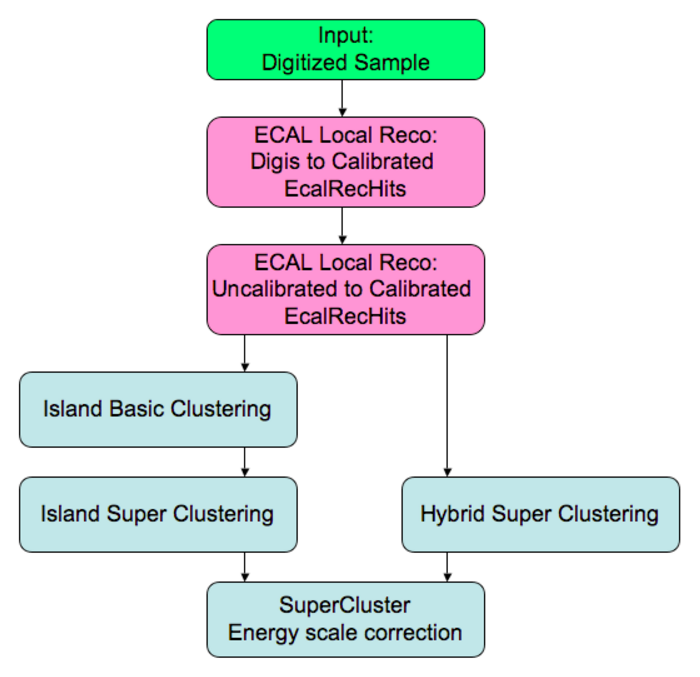
\includegraphics[width=10cm]{Chapter3/ECAL_Reco.png}
\caption{Various steps followed in reconstruction of particles inside ECAL.}
\label{fig:ECAL_Reco}
\end{center}
\end{figure}
\vspace{-0.3in}

\paragraph{Calibration of Ecal channels}\label{para:Calib}
\hspace{\parindent} The e$^{-}/\gamma$ signals in ECAL are calibrated and corrected to account for a number of detector effects~\cite{Chatrchyan:2013dga}.
The ECAL crystals have a tendency to degrade light response if illuminated continuously for a long time, therefore, the transparency of these crystals is
monitored during data taking by using a synchronous laser system and the observed changes are corrected for individual crystals during event reconstruction.
The relative calibration of individual channels is done by deploying the knowledge of $\phi$-symmetry of various energy depositions, the invariant mass of
$\pi^{0}/\eta$ mesons in diphoton channel and the momentum measurement of electrons, coming from decays of W$^{\pm}$ and Z bosons, in tracker.

\paragraph{Clustering}
\hspace{\parindent} The clustering algorithms group together the crystals associated with different electromagnetic showers into clusters.
Since the showers have a spread in $\phi$-direction due to the magnetic field, the clusters which
are close in $\eta$-direction are further grouped together into superclusters using a larger $\phi$ window.
Due to different crystal geometries in ECAL barrel and
endcap, two different algorithms, namely, Hybrid algorithm in barrel and Multi5$\times$5 (a modified island) algorithm in endcap, described in detail below are used. 

\vspace{-0.2in}
\begin{itemize}[leftmargin=*]
\item {\bf{Hybrid algorithm}}: The hybrid algorithm is a super-clustering algorithm deployed in the ECAL barrel that makes use of the $\eta-\phi$ geometry of crystals
  and the corresponding knowledge of lateral shower shape in $\eta$-direction to construct superclusters of electron and photon energy deposits.  This algorithm
  considers fixed length window in $\eta$ while variable length window in $\phi$-direction. An illustration of the algorithm has been provided in \fig{\ref{fig:Hybrid}}.
  
  \begin{figure}[h]
  \begin{center}
  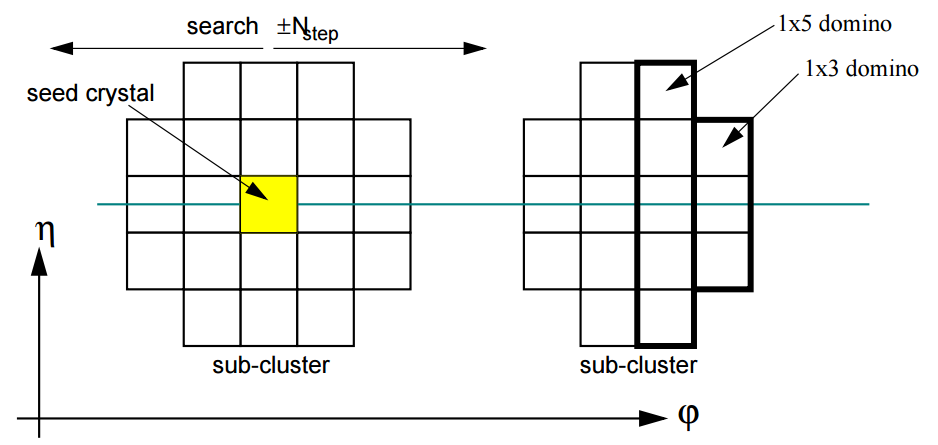
\includegraphics[width=13cm]{Chapter3/PhReco_hybrid_algo.png}
  \caption{An illustration of the Hybrid algorithm used for clustering in ECAL barrel region.}
  \label{fig:Hybrid}
  \end{center}
  \end{figure}
  \vspace{-0.2in}
The complete step-by-step procedure is outlined as follows:
  \begin{enumerate}
  \item Start by searching for a seed crystal, that is the maximum energy crystal satisfying $E_{\textrm{T}}$ $>$ $E_{\textrm{T,seed}}^{\textrm{thres}}$
    (1\unit{GeV}). The crystal should not belong to any other cluster. Terminate the process in case no such crystal is found.
  \item Construct a 1$\times$3 domino of crystals in $\phi-\eta$ direction. If $E_{\textrm{domino}}$ $>$ 0, then extend it to a 1$\times$5 domino. Add other 1$\times$5
    dominoes to it by moving in $\phi$-direction on either side of seed domino upto $\pm$N$_{\textrm{step}}$ crystal length in $\phi$ where N$_{\textrm{step}}$ = 17.
    If energy of a domino falls below $E_{\textrm{domino}}^{\textrm{thres}}$ (0.1\unit{GeV}), do not consider it.
  \item Group the selected adjacent dominoes into local energy clusters. If energy of a local cluster falls below $E_{\textrm{cluster}}^{\textrm{thres}}$ (0.35\unit{GeV}),
    then remove the corresponding dominoes from the final supercluster. 
  \end{enumerate}
\item {\bf{Multi5$\times$5 algorithm}}: Since the geometry of crystals in ECAL endcap is not the same as in the barrel, a different algorithm named Multi5$\times$5
  has been utilized in endcaps to collect the energy deposits within a window in $\eta-\phi$ plane.
  The Multi5$\times$5 algorithm first naively creates the basic clusters and then group them together into superclusters on the basis of their proximity in $\eta/\phi$
  direction. The complete description of the procedure is provided as follows:
  \begin{enumerate}
  \item At first, the seed crystals that do not belong to any cluster and that satisfy  $E_{\textrm{T}}$ $>$ $E_{\textrm{T,seed}}^{\textrm{thres}}$,
    required to be equivalent to 0.18 \unit{GeV}, are selected. Terminate the process if no such seed is found.
  \item The seeds are required to be local maxima when compared to the four direct neighbours. If this is not the case, repeat the previous step again.
    Arrange all the seeds in descending order of $E_{\textrm{T}}$.
  \item Start with the highest $E_{\textrm{T}}$ seed and move towards the lower ones while constructing 5$\times$5 crystal matrices around each.
    In this process, do not include the crystals in a matrix that have already been clustered in a previous matrix. The matrices in Multi5$\times$5 algorithm
    can partially overlap with each other
    but the crystals will only belong to the one with high $E_{\textrm{T}}$ seed. The overlapping
    matrices represent the close showers due to bremsstrahlung etc.
\item In order to construct a supercluster, all the 5$\times$5 clusters whose total energy satisfies, $E_{\textrm{T,cluster}}$ $>$      
  $E_{\textrm{T,cluster}}^{\textrm{min}}$ (1\unit{GeV}), are considered within a search road in $\eta$ and $\phi$ around each seed having the range $\eta\pm\Delta\eta$
  and $\phi\pm\Delta\phi$ where $\Delta\eta$ = 0.07 and $\Delta\phi$ = 0.3\unit{rad}. An illustration of this is presented in \fig{\ref{fig:Multi5x5}}.
  \end{enumerate} 
  \begin{figure}[h]
  \begin{center}
  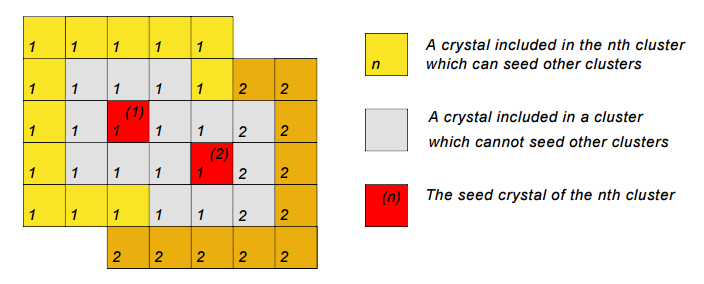
\includegraphics[width=11cm]{Chapter3/PhReco_multi5x5_algo.png}
  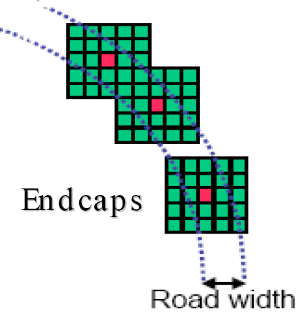
\includegraphics[width=4.5cm]{Chapter3/Multi5x5_road.png}
  \caption{An illustration showing overlapping of two Multi5$\times$5 clusters. Clusters in yellow are eligible to seed other Multi5$\times$5 clusters if
    they form the local energy maxima. The mechanism of formation of a supercluster using many multi5$\times$5 clusters is also shown.}
  \label{fig:Multi5x5}
  \end{center}
  \end{figure}
\end{itemize}
\vspace{-0.2in}

Since the pre-shower detector is present in front of ECAL endcaps in the $\eta$ range 1.65 $<$ $|\eta|$ $<$ 2.6, the particles deposit a fraction of their energy in the
pre-shower before reaching the endcap. In order to obtain this energy, the energy weighted positions of all the 5$\times$5 clusters belonging to a supercluster
in endcap are taken and extrapolated to the preshower planes, while taking the most energetic cluster as reference point.
The maximum distance between the clusters and the
reference point in $\phi$, along with an extension of $\pm$0.15\unit{rad}, is taken as the pre-shower clustering range in $\phi$. The corresponding range in $\eta$ has been
set to $\pm$0.15. The energy deposited in pre-shower in this range is computed and added into the endcap supercluster energy.

Each supercluster corresponds to a potential photon candidate.
The position of a supercluster in all the clustering algorithms is estimated via an energy weighted average of the positions of all the crystals belonging to the
supercluster. Each crystal is assigned a weight equivalent to, $w_{i} = max(0,4.7\,+\,\ln(E_{i}/E_{SC}))$~\cite{Meschi:687345}.
The supercluster position is then connected to the primary vertex of the event to obtain a direction of photon's momentum.
If many primary vertices exist in an event, then the one with highest track sum ${\ptx{2}}$ is considered.

\paragraph{Energy scale corrections of superclusters}
\hspace{\parindent} There are many factors that affect the resolution of the energy measured in ECAL using clustering algorithms.
These mainly include the energy losses due to the bremsstrahlung and photon conversions in the material of the tracker, leading to an underestimation of the energy.
The aim of supercluster energy corrections is to compensate for various energy losses and achieve a homogeneous response throughout the ECAL.\
The corrected energy of a reconstructed particle in ECAL is given by
\begin{equation}
E = F\times{G}\times\sum_{\textrm{cluster}}c_{i}\times{A_{i}}
\end{equation}
where $A_{i}$ refers to the signal amplitude given by the ADC counts; $c_{i}$ is the inter-calibration term that equalizes the different crystal's response
(as discussed under~\ref{para:Calib});
$G$ is the scale representing the global correction term defined such that the product of $G$ and energy amplitude of a $5\times5$ crystal matrix is equivalent to
the energy of an unconverted photon. The factor $F$ refers to the supercluster correction term and it includes corrections for three type of effects in barrel while
two type of effects in endcap, described as below:
\begin{itemize}[leftmargin=*]
  \setlength\itemsep{0.07em}
\item The factor $C_{\textrm{EB}}(\eta)$ used in barrel only to compensate for the lateral energy leakage from the exposed sides of the EB crystals.
\item The correction term $f_{\textrm{brem}}$ that is used to correct for the response of the clustering algorithms with different SC topologies
  towards the shower.
\item The residual correction term, $f(E_{\textrm{T}}, \eta)$, applied to all the reconstructed superclusters. It corrects for the non-linear
  matter distribution in the detector and the corresponding energy dependence.
\end{itemize}
\subsubsection{Photon identification}\label{Se:Ph_identi}
As photons are an important ingredient of many prominent physics searches, a precise identification and selection of photons is a crucial task of CMS physics
program. The photons selected using various reconstruction algorithms can have a significant fraction of fake photons coming from different sources.
In addition, the signal photons (directly coming from pp interactions) are contaminated with a large fraction of background photons (coming
from decay of other particles), arising mainly from the decay of neutral mesons (mainly, $\pi^{0}$ and $\eta$)
produced in the jets. These mesons decay into two photons which can get reconstructed as a single photon if the initial $\pt$ of mesons is quite high.
Two different algorithms for photon identification have been deployed in CMS: one approach considers the selections applied to the individual photon variables;
while second approach uses a multivariate technique.

The analysis documented in this thesis adopts the first approach that makes use of the different photon variables utilizing the knowledge of properties of photons.
These variables can be divided into two different categories as mentioned below:
\paragraph{Shower shape variables}
\hspace{\parindent} The direct photons are distinguished from background photons and other particles on the basis of their lateral shower patterns
within the calorimeter cells. A number of variables are utilized under this category, including
\vspace{-0.1in}
\begin{itemize}[leftmargin=*]
\item {\bf{Shower profile}}: Studying the lateral extension of energy deposits in the $\eta$-direction, is a very sophisticated and powerful way to distinguish
  the showers due to a single photon or two overlapping photons. A variable, \sigmaIetaIeta, is used that provides the transverse shape of EM cluster in
  a particular $\eta$ direction  and is defined as the energy weighted standard deviation
  of a single crystal $\eta$ in a matrix of $5\times5$ crystals centered around the maximum energy crystal.  It is computed using logarithmic weights and is defined as:
\begin{equation}
\begin{split}
\sigma_{i{\eta}i{\eta}}^{2} =  &\frac{{\sum_{5\times5}}(\eta_{i}-\bar{\eta})^{2}w_{i}}{{\sum}w_{i}}, \\
                           &\textrm{where}\:\:\bar{\eta} = \frac{{\sum}w_{i}\eta_{i}}{{\sum}w_{i}} \:\:\: \textrm{and} \:\: w_{i} = \textrm{max}\left[0 \: ;\: 4.7+\textrm{log}\left(\frac{E_{i}}{E_{5\times5}}\right)\right].
\end{split}
\end{equation}
Here the distances $\eta$ are measured in units of crystal size in the $\eta$-direction. This variable has a symmetric and narrow distribution for a
prompt photon while has a long tail on the lower side of the distribution for misidentified or overlapping photons.
Another variable, \sigmaIphiIphi, a counterpart of \sigmaIetaIeta in
$\phi$ direction is also used, however, it is less effective compared to \sigmaIetaIeta. 
\item {\bf{Single tower hadronic over electromagnetic ratio (H$/$E)}}: It is defined as the ratio of energy deposited in the single HCAL tower, closest to
  the photon supercluster position and centered in the photon direction, within a cone of radius $R$ = 0.15 in $\eta-\phi$ plane and the energy deposited by that supercluster in
  the ECAL. Due to the large depth of ECAL ($\sim$ 26$X_{0}$), the probability of EM shower leakage in HCAL is relatively small, so this variable proves to be a
  good discriminator. 
\item {\bf{R$_{9}$}}: It is defined as the ratio of total energy deposited in a 3$\times$3 crystal matrix around the most energetic crystal in a supercluster and
  the total supercluster energy. The energy spread due to a pair of overlapping photons is larger as compared to a single photon, therefore, this variable
  also provides a good discrimination. 
\item {\bf{Conversion safe electron veto}}: This variable is used to distinguish between electrons and converted photons. It requires that for a photon cluster
  in ECAL, there should not be any charged particle track with pixel hits, matching with the conversion vertex, in the tracker pointing towards the photon direction. 
\end{itemize}
\paragraph{Isolation variables}
\hspace{\parindent} If a photon candidate is a direct descendant of a pp collision, it will be quite away from other particles produced in the same collision.
On the other hand, if a photon is a decay product of a hadronic jet, it will be associated with hadronic activity in its vicinity.
Therefore, requiring limited amount of activity around the photon results into extraction of good photon candidates. Various isolation sums, expressed
as the total energy$/$momentum carried by various particles within a specific volume around the photon candidate, are estimated using the particle flow (PF)
algorithms~\cite{Sirunyan:2017ulk}, making use of all the sub-detectors. These sums are evaluated within a cone of radius $R$ = 0.3 around the photon candidate while
neglecting the energy$/$momentum within a veto region of smaller radius, to avoid the inclusion of the candidate photon energy.
Three different isolation sums depending upon the
type of particles under consideration, are defined:
%\vspace{-0.05in}
\begin{itemize}[leftmargin=*]
\item {\bf{PF charged hadron isolation}}: $\sum{\pt}$ of all the charged hadrons within a hollow cone of 0.02 $<$ $R$ $<$ 0.3 around the photon supercluster.
\item {\bf{PF neutral hadron isolation}}: $\sum{\pt}$ of all the neutral hadrons within a cone of $R$ = 0.3 around the photon supercluster. 
\item {\bf{PF photon isolation}}: Scalar $\sum{\pt}$ of all the photons within a cone of $R$ = 0.3 while excluding a strip in $\eta$ of 0.015 around
  the photon supercluster.
\end{itemize}
\subsection{Jet reconstruction and identification}
Jets in the detector represent the experimental signature of quarks and gluons emerging from the high energy pp collision.
Since, quarks and gluons can not survive individually
owing to their colour confinement, they hadronize in the form of jets soon after their production. Therefore, jets provide a way to access and study the
underlying processes at partonic level. A precise determination of jets and understanding of their properties is of utmost importance for many physics searches.

Jets are made up of a large number of particles including leptons, hadrons as well as bosons (mainly photons). Within the detector, these appear as a collimated spray of
particles in a particular direction as seen in \fig{\ref{fig:Jet}}. As they travel through the detector, they leave their signals in different detector components.
These signals are then combined by the jet reconstruction algorithms to build a jet. A number of jet energy corrections are also considered to equalize
the reconstructed jet energy to the true particle-level energy.

\begin{figure}[h]
\begin{center}
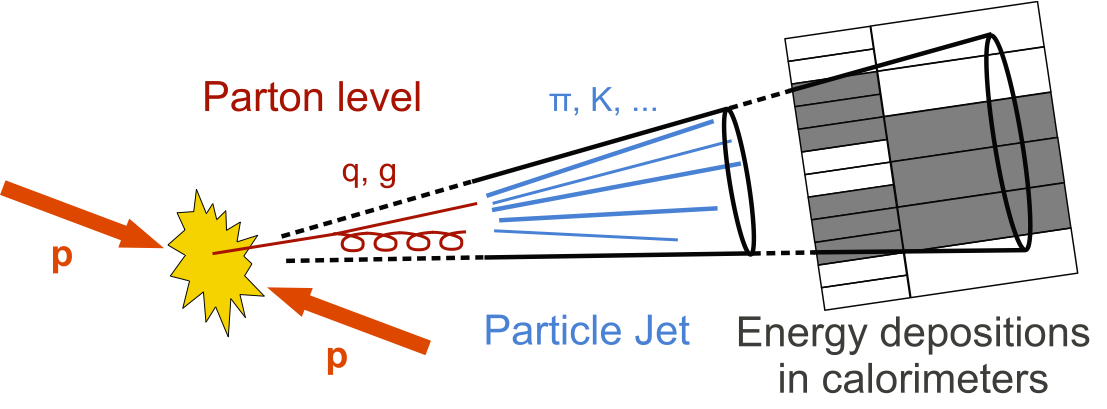
\includegraphics[width=13cm]{Chapter3/Sketch_Jet.png}
\caption{A pictorial representation of a jet.}
\label{fig:Jet}
\end{center}
\end{figure}
\vspace{-0.2in}

\subsubsection{Jet reconstruction}
The aim of jet reconstruction is to reconstruct and identify jets coming from the hadronization of partons.
This process can be divided into two parts: The first part reconstructs the individual jet constituents and the second part clusters
them together to produce a complete jet. 

For reconstruction of jet constituents, three different approaches are considered at CMS: a calorimeter based approach which utilizes the
information of the calorimeter energy deposits only; a Jet$-$Plus$-$Track (JPT) approach that improves
the calorimeter information by using the additional knowledge from the associated tracks; a Particle-Flow (PF) approach that attempts to combine the information
from all the relevant sub-detectors. A highly improved spatial and momentum resolution can be achieved by the use of PF approach
as compared to calorimeter or JPT approach. 

The jet clustering algorithms are used to cluster individual jet constituent particles to form a jet. These algorithms can be broadly divided into
two classes: the sequential recombination algorithms and the cone algorithms. The sequential algorithms work by combining a pair of particles based on the
closeness in some distance measure and then repeating the procedure for other particles until some stopping condition is reached. The main sequential algorithms
employed at CMS include, \kt~\cite{Catani:246812}, \antikt~\cite{Cacciari:2008gp} and Cambridge$/$Aachen (CA)~\cite{CMS-PAS-JME-09-001, Dokshitzer:1997in},
described by the distance measurements,
\begin{equation}
  \begin{split}
    & d_{ij} = \textrm{min}(k^{2p}_{\mathrm{T}i}, k^{2p}_{\mathrm{T}j}) \frac{\dR^{2}_{ij}}{R^{2}} \hspace{0.2in} \textrm{and}\\
    & d_{iB} = k^{2p}_{\mathrm{T}i},
  \end{split}   
\end{equation}
where, \\
$d_{ij}$: distance between $i$th and $j$th particle, \\
$d_{iB}$: distance of $i$th particle from the beam line, \\
$k_{\mathrm{T}}$: particle's transverse momentum, and \\
$\dR_{ij}$: spatial distance between $i$th and $j$th particles, $\sqrt{(\eta_{i} - \eta_{j})^{2} + (\phi_{i} - \phi_{j})^{2}}$. \\
The parameter $R$ determines the angular reach of a jet and is usually called the jet radius. The parameter, $p$ = 1 for \kt algorithm,
implies that this algorithm clusters the soft particles (low \pt) first, $p$ = $-1$ for \antikt algorithm
means that it clusters hard particles (high \pt) first and $p$ = 0 for CA algorithm performs an energy independent clustering. 
On the other hand, the cone algorithms define specific conical regions around the particles and put together all the particles inside the cone in the form of a jet 
such that the total momentum of the particles coincide with the cone axis. The famous cone algorithms include,
Iterative cone, Midpoint cone, SIScone etc. These algorithms mainly differ from each other in the strategy used to search for the stable conical region. 
The \fig{\ref{fig:JetClusterAlgo}} represents the behaviour of different jet clustering algorithms.
\begin{figure}[h]
\begin{center}
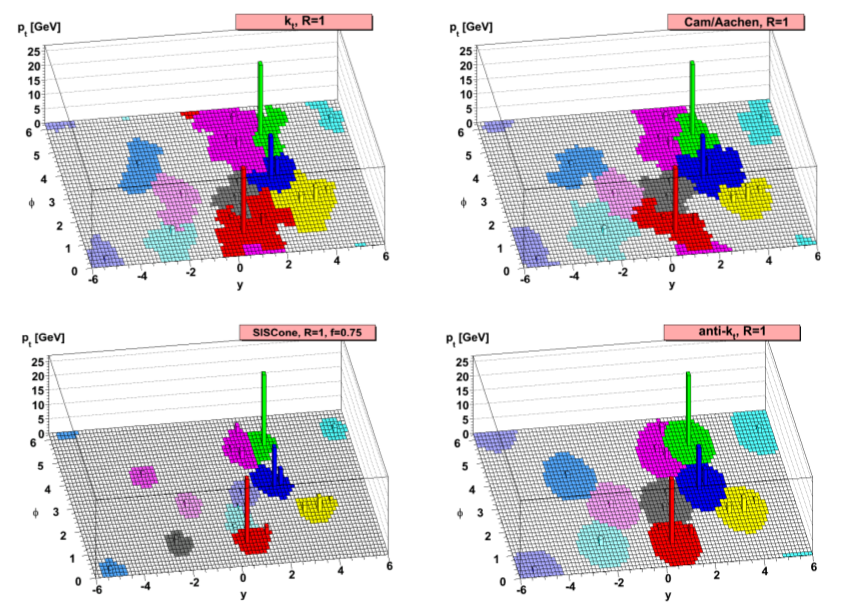
\includegraphics[width=13cm]{Chapter3/JetClusteringAlgo.png}
\caption{The behaviour of different jet clustering algorithms.}
\label{fig:JetClusterAlgo}
\end{center}
\end{figure}
%\vspace{-0.2in}

The sequential algorithms have a number of advantages over the cone algorithms, like: simplicity and detector independence, can be easily implemented in experimental
analyses and theoretical calculations, insensitive to hadronic effects, infrared and collinear safe\footnote{Infrared safety requires that the clustering
  algorithms should not be affected by the inclusion of an extra soft gluon and collinear safety requires that the jet clustering should remain same for
  splitting of a parton into two partons. Both of these lead to finite perturbative calculations upto any order.} etc.
The analysis in this thesis considers the particle flow jets clustered using the \antikt algorithm. A detailed description of these has been provided below:

\noindent
\underline{\bf{Particle flow reconstruction algorithm}}:
The particle flow algorithm of CMS~\cite{Sirunyan:2017ulk, CMS-PAS-PFT-09-001} relies mainly on the high efficiency of track reconstruction and fine granularity
of ECAL and HCAL. This algorithm works by linking the energy clusters in the calorimeters with the tracker signals to create a complete picture of the event.
Since, this algorithm reconstructs individual particles corresponding to each sub-detector first, a dedicated calibration can be done and the impact of
non-compensating nature of HCAL can be mitigated to get an overall good response. Also due to the availability of tracking and vertex information,
the impact of pile-up collisions can be reduced. The list of individual particles from each sub-detector is then used to reconstruct jets, \met, $\tau$, b-jets etc. 

This algorithm is performed in three main steps. The first step builds the basic elements of PF algorithm, like the
reconstruction of charged particles tracks in the tracker and energy clusters in the
calorimeters. The energy clustering in HCAL starts by searching for a seed channel, a local energy maxima. The topological clusters are then formed by adding neighbouring
channels to it. The energy of each calorimeter channel is required to be above some predefined threshold, in order to avoid any contributions from electronic noise etc.
The energies and positions of the final clusters are determined using an iterative method by re-weighting the contributions of individual channels
on the basis of their distance from the seed channel. 
This step is then followed by a second step that involves the building of PF blocks using a mechanism known as link algorithm, which performs the
linking of the tracks with the energy deposits in ECAL and HCAL, compatible with the electromagnetic and hadronic shower profiles.
A link between ECAL and HCAL energy deposits is also made if the ECAL cluster position lies within the envelope of HCAL cluster. The tracks are also linked to
the muon hits in the muon system, thereby forming global muons. The resultant PF block consists of a maximum of three elements.
The quality of these blocks is determined by the compatibility of its elements, either in the form of $\eta-\phi$ distance in case of track$-$to$-$cluster and
cluster$-$to$-$cluster links or in the form of $\chi^{2}$ fit in case of track$-$to$-$muon links. The third step consists of the reconstruction of final PF objects on the
basis of the PF blocks.

The performance of PF algorithm has been studied using simulated events~\cite{CMS-PAS-PFT-09-001}. A great precision is achieved, using tracker and ECAL,
for the measurement of around 90$\%$ of jet energy taken by the charged hadrons and photons.
The remaining 10$\%$ of jet energy shared by neutral hadrons is measured solely in HCAL and 
has an energy resolution of 120$\%/\sqrt{E}$.

\noindent
\underline{\bf{\boldmath{$\Antikt$} clustering algorithm}}:
The default jet clustering algorithm used in CMS is one of the sequential recombination algorithm, the \antikt~\cite{Cacciari:2008gp} algorithm.  
It determines two distance measures for a pair of particles ($i,j$) as
\begin{equation}
  \begin{split}
    & d_{ij} = \textrm{min}(k^{-2}_{\mathrm{T}i}, k^{-2}_{\mathrm{T}j}) \frac{\dR^{2}_{ij}}{R^{2}} \hspace{0.2in} \textrm{and}\\
    & d_{iB} = k^{-2}_{\mathrm{T}i}.
  \end{split}   
\end{equation}
This algorithm works by finding the distance of $i$th particle from the closest $j$th particle ($d_{ij}$) and from the beam line ($d_{iB}$), by using
the definition of distance measures given above. If $i$th particle is closer to $j$th particle as compared to beam line ($d_{ij}$ is smallest),
it replaces $i$th and $j$th
particle with a single new particle of momentum $k_{\mathrm{T}i}+k_{\mathrm{T}j}$, often called a pseudojet, as it is neither a single particle nor a full jet.
However, if the $i$th particle is closer to beam line as compared to $j$th particle ($d_{iB}$ is smallest), then it removes the $i$th particle from the
list of particles under study and considers $i$th particle as an inclusive jet. The
algorithm then repeats this procedure with a new pair of closest particles$/$pseudojets, until it includes all the particles. The CMS uses \antikt algorithm
corresponding to two values of jet radius, viz 0.4 and 0.8, forming AK4 and AK8 jets.
\subsubsection{Jet energy corrections}\label{Se:JetEnCorr}
The energy of a reconstructed jet is not the same as that of the true energy of a particle level jet. The primary reason being the non-linearity and non-uniform
response of calorimeters, especially HCAL.    
The jet energy corrections (JEC)~\cite{CMS-PAS-JME-07-002} are a set of tools that performs the mapping of the reconstructed jet energy to the actual particle-level energy.
At CMS, a multi level factorized approach to JEC has been considered where each level correspond to a different correction of specific type. These corrections
are extracted using the data-driven as well as the simulation methods and are provided as $\textit{in-situ}$ calibrations in data and MC.  
Each correction level is dependent on various jet quantities and provides a scaling to the jet four momentum\footnote{($p_{x}, p_{y}, p_{z}, E$)}.
These corrections are always applied sequentially in a fixed order. The different JEC levels are represented in \fig{\ref{fig:JEC_levels}} and are described below:
\begin{figure}[h]
\begin{center}
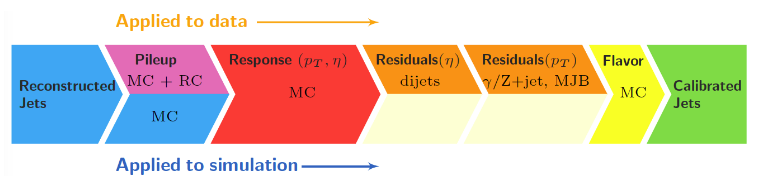
\includegraphics[width=15cm]{Chapter3/JES_diagram.png}
\caption{Different jet energy correction levels applied to data and MC.}
\label{fig:JEC_levels}
\end{center}
\end{figure}
\vspace{-0.4in}
\begin{itemize}[leftmargin=*]
\item {\bf{L1 Offset}}: The purpose of the L1 correction is to subtract any energy contribution coming from the pile-up and underlying events~\cite{Cacciari:2007fd}.
  This correction, in principle, removes the dependence of data sample on the luminosity, so that the further corrections are applied on a
  luminosity independent sample. These corrections are estimated using the events processed with and without considering pile-up overlay in a simulated
  sample of QCD dijet and parameterized as a function of energy density $\rho$, jet area, $\eta^{\textrm{jet}}$ and $\pt^{\textrm{jet}}$. The residual differences between
  data and simulation are corrected as a function of $\eta$ using a random cone method implemented using zero-bias events, resulting into different L1 corrections for
  data and MC.
\item {\bf{L2 Relative}}: These corrections are applied to both data and MC to make the jet response uniform as a function of pseudorapidity, $\eta$.
\item {\bf{L3 Absolute}}: After correcting the jet response in $\eta$, it is also made uniform in $\pt$ using L3 corrections. The L2 and L3 corrections are now
  computed together using QCD dijet samples and are collectively called L2L3 MC-truth corrections.
\item {\bf{L2L3 Residual}}: This correction is determined by the $\textit{in-situ}$ measurements of absolute and relative jet energy scales and is meant to
  correct the small differences between data and MC, of the order of a few $\%$, in jet response. A correction factor, equivalent to the residual difference
  between data and MC, is applied only to data. 
\end{itemize}
Apart from these, an optional L5 flavor correction derived using Z$+$jet and $\gamma+$jet simulated samples, is also applied in some cases. The analysis in this thesis
considers the essential L1, L2, L3 and L2L3 corrections only. Each correction level also has the related uncertainties, forming the biggest source of systematic error
in a jet measurement. 
\subsubsection{b-tagging of a jet}\label{Se:Jet_btagging}
The jets arising from the hadronization of b-quarks are known as b-jets. The b-jets have many distinctive signatures (\fig{\ref{fig:bjet}}) like,
long lifetime ($\sim$ $10^{-12}$\unit{s}),
large mass (4.2\unit{GeV}), high track multiplicity ($\sim$ 4$-$5), relatively large semi-leptonic branching ratio ($\sim$ 20$\%$ for each of $e^{-}$ and $\mu^{-}$), hard
fragmentation function\footnote{A significant fraction of initial b-quark's momentum is taken away by b-hadrons.} etc., which leads to their precise
measurement. The CMS with its rigorous charged particle tracking, powerful lepton identification and highly segmented calorimetry, is well matched for the task
of b-jet identification~\cite{Chatrchyan:2012jua, Sirunyan:2017ezt}. The b-tagging is a kind of reconstruction procedure that utilizes 
various b-hadron properties and based on these, assigns a ``likelihood'' to each jet, of the presence of b-hadrons.
\begin{figure}[h]
\begin{center}
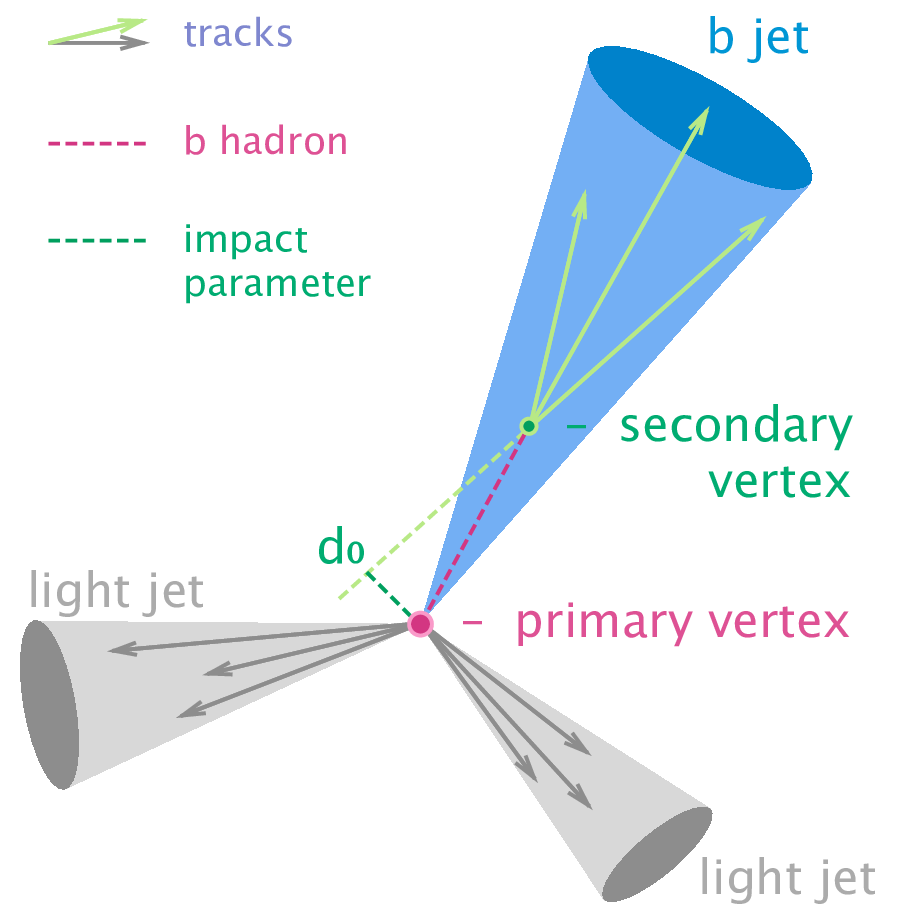
\includegraphics[width=5cm]{Chapter3/bjet.png}
\caption{A depiction of a b-jet emerging from the primary vertex.}
\label{fig:bjet}
\end{center}
\end{figure}


\begin{figure}[h]
\begin{center}
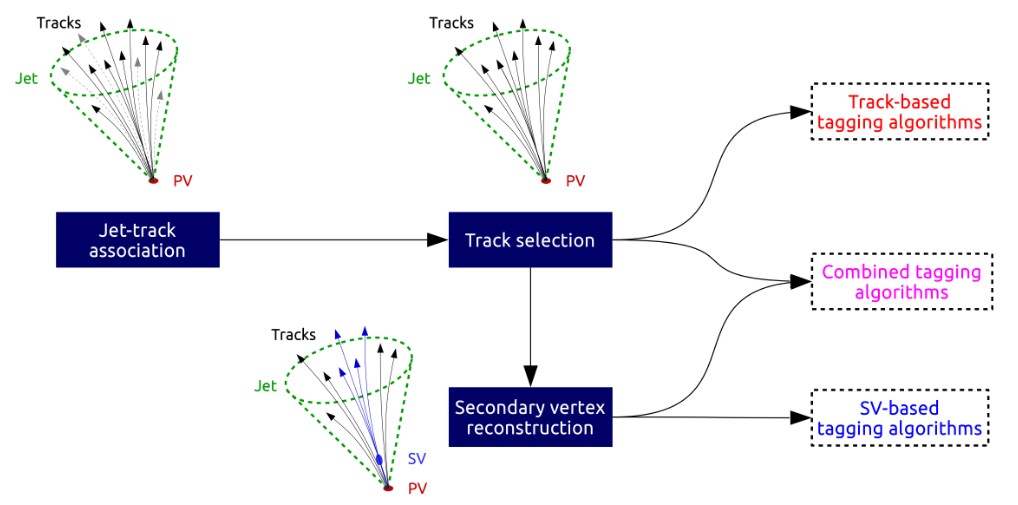
\includegraphics[width=15cm]{Chapter3/btagAlgorithms.png}
\caption{An illustration of b-tagging algorithms.}
\label{fig:bjetAlgo}
\end{center}
\end{figure}

A number of b-tagging algorithms have been deployed at CMS that mainly differs in their complexity and input information. All these algorithms provide a numerical
discriminator for a jet in the output whose value determines the b-tagging status of the jet. The higher is the value of discriminator, the larger is the probability of
the jet being a b-jet. These b-tagging algorithms are constructed on the basis of the information gathered from either the tracks or secondary vertex or soft lepton or
any combination of these, as presented in \fig{\ref{fig:bjetAlgo}}.
The main b-tagging algorithms employed in CMS are:
%\vspace{-0.1in}
\begin{itemize}[leftmargin=*]
\item {\bf{Track Counting (TC) algorithm}}: This approach exploits the long lifetime of b-hadrons and considers the charged tracks associated with it.
  It computes the significance of the signed impact parameter\footnote{Impact Parameter (IP) is defined as the minimum distance between the track and primary vertex, the
    sign of IP is determined by the scalar product of IP segment with the jet direction.} of all the good tracks, arrange them in decreasing significance and assign the
  significance of $N$th track to the discriminator. It leads to an algorithm of high efficiency for $N$ = 2 and high purity for $N$ = 3. 
\item {\bf{Jet Probability (JP) algorithm}}: This algorithm uses information from all selected tracks in a jet. Using a sample of tracks with
  negative impact parameters, it builds a probability distribution
  function (PDF) that considers the probability of a track to be originating from the primary vertex. Based on this PDF, a probability pointer is assigned to each
  track and a discriminator is built using full set of tracks. A version of JP algorithm, known as jet B probability is also used that considers only the four
  highest displaced tracks matching with the reconstructed multiplicity of the b-hadron decay vertex. 
\item {\bf{Soft Lepton (SL) algorithm}}: This algorithm identifies the b-hadrons on the basis of their semi-leptonic decays as the leptons from b-decay usually tend
  to have high \pt relative to the jet axis. The corresponding b-tag discriminator is the result of the neural network\footnote{A neural network
    is a hardware$/$software system designed on the basis of working of neurons in the human brain.} build up using lepton \pt, impact parameters
  and some other variables.
\item {\bf{Simple Secondary Vertex (SSV) algorithm}}: This algorithm considers the reconstruction of secondary vertex from the b-hadron decay using an adaptive
  vertex finder technique and uses the variables associated with it to compute the discriminator value.
\item {\bf{Combined Secondary Vertex (CSV) algorithm}}: This is the most sophisticated and complex approach making use of all the known information like
  secondary vertices, lifetime, IP significances, decay lengths etc. This algorithm has the capability to provide a discrimination even when no secondary vertex is
  reconstructed. It uses a list of variables and feeds them as input into a likelihood ratio which is then used to compute the discriminator value.
  A ``version 2'' of this algorithm known as ``CSVv2'' has
  also been introduced during LHC Run II that makes use of the artificial neutral networks instead of likelihood ratio.   
\end{itemize}
\vspace{-0.2in}
These algorithms have a b-tag identification efficiency varying in a range of $40-70\%$. These are available in three working points:
loose, medium and tight, corresponding to light flavour mis-tagging rate of 10$\%$, 1$\%$ and 0.1$\%$, respectively.
At CMS, these algorithms are determined using the inclusive multijet, muon enriched jets and dilepton $t\bar{t}$ data samples,
the jets are required to be PF jets clustered using \antikt algorithm having a \pt $>$ 20\unit{GeV} and lying within the tracker acceptance region, $|\eta|$ $<$ 2.4. 
\subsubsection{Jet identification}\label{Se:JetID}
The reconstructed and calibrated jets contain a significant fraction of fake jets coming mainly from the electronic noise and other detector artifacts.
In order to identify and locate a good collection of jets to be used in an analysis, a set of identification variables are defined~\cite{Web:JetId}, listed as below:
\vspace{-0.1in}
\begin{itemize}[leftmargin=*]
  \setlength\itemsep{0.1em}
\item {\bf{Charged hadron fraction}}: The fraction of energy deposited in HCAL by charged hadrons.
\item {\bf{Neutral hadron fraction}}: The fraction of energy deposited in HCAL by neutral hadrons.
\item {\bf{Charged electromagnetic fraction}}: The fraction of energy deposited in ECAL by charged constituents of the jet.
\item {\bf{Neutral electromagnetic fraction}}: The fraction of energy deposited in ECAL by neutral constituents of the jet.
\item {\bf{Number of constituents}}: The number of particles in a jet.
\item {\bf{Charged multiplicity}}: The number of charged particles in a jet.
\end{itemize}
\vspace{-0.1in}
\section{Event Simulation}
Event simulation is an integral part of any high energy physics experiment right from the designing stage to the final analysis.
It is almost impossible to perform a physics analysis without the use of simulated data. It acts as a reference to the detector output as well as
allows us to study the behaviour and consequences of any new theory without having observed it directly. 
The various efficiencies and correction factors used by the analyses are computed by comparing experimental and simulated data while a number of
systematic uncertainties are computed using simulated data alone. In general, the quality of any physics result is strongly
influenced by the quality of simulation involved. 

Event simulation produces events that perfectly mimic the output from an actual detector. The various steps involved in a simulation chain are presented schematically
in \fig{\ref{fig:SimChain}}. 
\begin{figure}[h]
\begin{center}
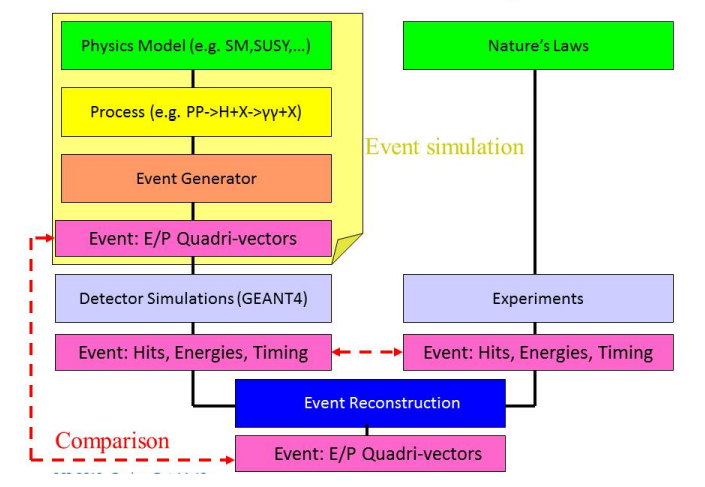
\includegraphics[width=15cm]{Chapter3/SimulationChain.png}
\caption{Event simulation and data analysis chain.}
\label{fig:SimChain}
\end{center}
\end{figure}
%\vspace{-0.2in}

As the first step of the simulation chain, the ``Physics Model'' in which the calculation has to be performed, is selected. The physics model can be the
standard model (to simulate background processes) or any model beyond the standard model (to simulate signal processes of new physics).  
The simulation process is defined at the next level by specifying the input$/$output particles and the order of calculation. The expressions for matrix element and
probability cross-section are prepared automatically on the basis of the selected physics model.   
At the ``Event Generator'' level, the matrix element is integrated over the entire phase space and the random samples of all final state particles, along with
the information of their energy-momentum, are generated. The generated events are then made to propagate through a ``Detector Simulation'' model
that represents the simulation of an actual detector.    
The huge amount of information produced in output by the detector simulation exactly replicate the output from a real detector. At this level,
both the theoretical simulated data and experimental detector data are at equal footing and can be compared with each other. The simulated data
is reconstructed using the same reconstruction programme as used for real data. Comparison of reconstructed simulated data with real data
provides a test of self-consistency of the underlying physics model, though any discrepancy between the two may hint towards some new physics. 
The final analysis is performed using a data analysis toolkit, known as ROOT~\cite{Brun:1997pa}. The simulated and observed events passing various
filters and cuts are studied and compared by organizing them in the form of histograms. At CERN, the simulation and analysis of data is performed using
a data distribution grid system known as WLCG (Worldwide LHC Computing Grid)~\cite{WLCG}. This infrastructure is based on the tiers
computing centers, distributed all around the world.

The two main components of event simulation process, viz, event generation and detector simulation are described in more detail in the sections below.
\subsection{Event generation}
Event generation~\cite{Buckley:2011ms, Dobbs:2004qw} is the first stage of the simulation process.
It is based on software programs that use Monte Carlo (MC) methods~\cite{robert2004monte, MC_Tech} to simulate events.
A Monte Carlo technique is basically an integration tool based on random sampling\footnote{A method of selecting a sample from a large statistical population such that
  each sample in the population has some predefined probability of being selected.}. It is mainly used to obtain approximate numerical solutions
of the analytical problems which are otherwise too complicated to solve. 

The main objective of event generators is to accurately provide the description of an actual particle collision.
In a high energy pp collision, the formation of a single event involve several steps as depicted in \fig{\ref{fig:EvtGen}}. At the start, the two partons
are selected, in flavor as well as in color, from each of the two colliding protons. These partons are allowed to radiate gluons, known as initial state radiation,
before interacting. The hard scattering process occurs upon interaction and results into the production of two or more final state particles, probably via a
resonance state. These final state particles can further decay into other particles producing
several daughters. The remaining quarks and gluons undergo the emission of parton showers before the final hadronization stage occurs, resulting into the
recombination of partons to form hadrons. In addition to these, the left over partons (known as beam remnants) of a proton,
after the parton underwent hard scattering is pulled off, can interact with each other, leading to the multiple parton interactions (MPI).
These MPIs result into creation of multiple vertices as well as addition of extra tracks and energy deposits interfering with the main collision,
referred to as the underlying events (UE). 
\begin{figure}[h]
\begin{center}
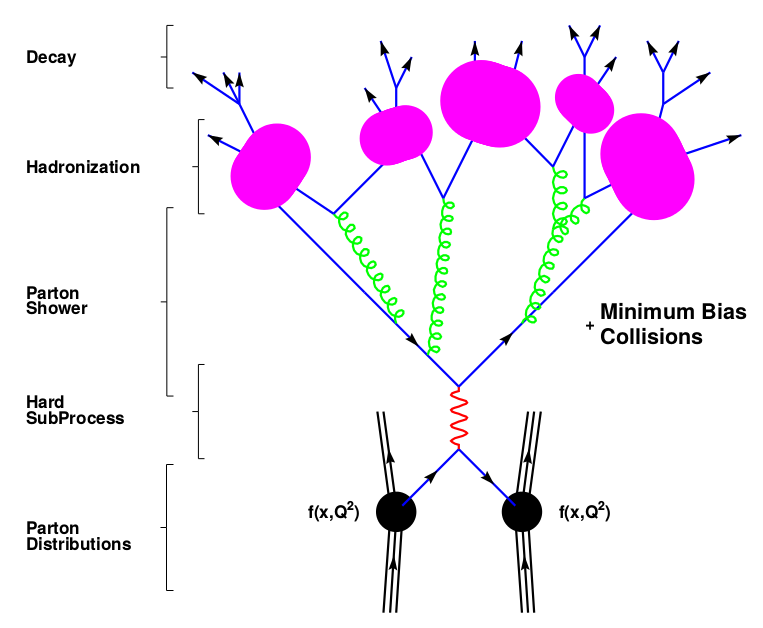
\includegraphics[width=13cm]{Chapter3/EventGeneration.png}
\caption{Sequential steps involved in the formation of an event.}
\label{fig:EvtGen}
\end{center}
\end{figure}
%\vspace{-0.2in}

The event generators also formulate an event in the same sequence through the use of different theoretical models for different physics aspects, like
hard and soft interactions, initial$/$final state parton showers, parton distribution functions, multiple interactions, underlying events,
parton hadronization and decay etc. Simulating these aspects of a process require the calculation of relevant matrix element involving loop
diagrams up to many orders, achieved by the use of dedicated MC techniques.

The cross-sections for various processes are stored within the event generators which are solved by the use of MC integration techniques.
The cross-section of a $2\rightarrow2$ process at tree-level is given by,
\begin{equation}
\sigma(ab\rightarrow{cd})=\sum_{ab}\int_{0}^{1}\int_{0}^{1} \hat{\sigma}_{ab\rightarrow{cd}}
            \left(\hat{s},\alpha_{s}(\mu_{R}^{2}),\frac{Q^{2}}{\mu_{F}^{2}},\frac{Q^{2}}{\mu_{R}^{2}}\right)f_{a}(x_{1},\mu_{F}^{2})f_{b}(x_{2},\mu_{F}^{2})dx_{1}dx_{2} 
\label{eq:gamJetXS}
\end{equation}
Here $Q$ is the scale of hard interaction while $\mu_{F}$ and $\mu_{R}$ are factorization and renormalization scale. 
The quantity, $\hat{s}=x_{1}x_{2}s$, $s$ is the center-of-mass energy of collision, $x_{1}$ and $x_{2}$ are the fractions of total proton's momentum, carried by two
interacting partons. The functions $f_{a}(x_{1},\mu^{2}_{F})$ and $f_{b}(x_{2},\mu_{F}^{2})$ are the probability density function for two partons,
also known as parton distribution function (PDF)~\cite{Martin:2009iq},
representing the probability of carrying a momentum fraction $x_{1}$ and $x_{2}$ by parton $a$ and $b$ respectively.
The initial partons for a hard interaction are selected by the use of PDF.
These PDF's are determined experimentally from deep inelastic scattering processes, Drell-Yan processes, and jet production at high energies.
The $\hat{\sigma}$ is the parton level cross-section of the sub-process $ab\rightarrow{cd}$.
The expression is integrated using MC techniques over the entire phase space.
If the expression contains loop corrections, then integration over loop propagators is also performed. The multi-dimensional integration
yield the total cross-section of the process. The event after passing through the various event generation levels is then
passed to the detector simulation stage.
\subsubsection{MC event generators}
A number of event generators based on MC techniques are used in present day colliders. These can be divided into general-purpose generators and specific generators.
The specific generators are good for simulating any particular physics aspect but need to be interfaced with general-purpose generators to simulate a complete
event. Examples of some of the general-purpose generators are: \pythia~\cite{Sjostrand:2014zea}, \madgraph~\cite{Alwall:2014hca},
$\herwigpp$~\cite{Bahr:2008pv}, \alpgen~\cite{Mangano:2002ea} and \sherpa~\cite{Gleisberg:2008ta}. The analysis
documented in this thesis uses \pythia and \madgraph as the generators to simulate various signal and background processes. A brief description of these
are given below.
\paragraph{\pythia}
\hspace{\parindent} It is one of the oldest general-purpose event generator used for lepton as well as hadron colliders.
Its hadronization model is based on the Lund string model~\cite{Sjostrand:1986hx},
consisting of around 240 hard scattering processes. It is a leading order (LO) event generator and
considers only two particles in initial and final states. It consists of models for initial and final state parton showers, hard processes matching and
merging, multi parton interactions, underlying events etc. It also has the facility to interface with external programs. 
\paragraph{\madgraph}
\hspace{\parindent} \pythia is an ideal event generator for simulating $2\rightarrow{2}$ processes, but in actual collisions, most of the processes contain
more than two particles in final state. The \madgraph~\cite{Alwall:2014hca} matrix element generator has the capacity to produce the processes with up to
nine particles in the final state. It uses ALOHA package~\cite{deAquino:2011ub} to automatically generate the amplitudes of relevant sub-processes.
The events simulated using \madgraph are put in some standard event format files known as Les Houches format files (LHE files)~\cite{Alwall:2006yp} which
are then passed to \pythia to simulate parton showering and hadronization. The \pythia also performs matching and merging of the matrix elements (ME)
with the partons showers (PS) using CKKW algorithm~\cite{Krauss:2002up} and MLM scheme~\cite{Mangano:2001xp}.
\subsection{Detector simulation}
In order to simulate the behaviour of particles within the detector, a software based model representing a virtual detector has been used.
The event generator output is made to pass through this detector simulation model to obtain a replica of actual collision data.
With increase in complexity and resolution of the detectors, the detailed simulation of an experimental setup has become a challenging task. It
requires efficient and sophisticated tools to accurately reproduce the behaviour of detector in the presence of collision particles.

In CMS, the simulation of the detector is performed using an object oriented toolkit known as \geant~\cite{Agostinelli:2002hh}.
The \geant consists of a set of C$++$ libraries
which can be used to simulate any detector system. It simulates the particle interactions in matter on the basis of Monte Carlo methods. 
The \geant package provide accurate description of various detector aspects like, detector geometry, material of different detector components and the
dead material such as bolts, cables, support etc. It consists of a set of physics models that are able to handle the various particle's interactions with
the matter over a wide range of energy, ranging from few hundred $\unit{eV}$s to \unit{TeV}. Starting from the event generator output, the events are made
to propagate through the detector simulation while taking into account the magnetic field for charged particles as well as the various interactions of
particles with matter like bremsstrahlung, multiple scattering, photon conversions, scintillation, ionization, cherenkov light etc.
Finally, the raw output similar to that of the actual detector data is obtained. 

